\section{Descriptive statistics}
\label{sec:stats_descriptives}

The first step in any statistical analysis should be to describe,
charaterize and importantly, visualize your data.  The normal
distribution (aka Gaussian or bell curve) lies at the heart of much of
formal statistical analysis, and normal distributions have the tidy
property that they are completely characterized by their mean and
variance.  As you may have observed in your interactions with family
and friends, most of the world is not normal, and many statistical
analyses are flawed by summarizing data with just the mean and
standard deviation (square root of variance) and associated
signficance tests (eg the T-Test) as if it were normally distributed
data.

In the exercise below, we write a class to provide descriptive
statistics of a data set passed into the constructor, with class
methods to pretty print the results and to create a battery of
standard plots which may show structure missing in a casual analysis.
Many new programmers, or even experienced programmers used to a
proceedural environment, are uncomfortable with the idea of classes,
having hear their geekier programmer friends talk about them but not
really sure what to do with them.  There are many interesting things
one can do with classes (aka object oriented programming) but at their
hear they are a way of bundling data with methods that operate on that
data.  The \texttt{self} variable is special in python and is how the
class refers to its own data and methods.  Here is a toy example

\begin{lstlisting}

In [115]: class MyData:
   .....:     def __init__(self, x):
   .....:         self.x = x
   .....:     def sumsquare(self):
   .....:         return (self.x**2).sum()
   .....:     
   .....:     

In [116]: nse = npy.random.rand(100)

In [117]: mydata.sumsquare()
Out[117]: 29.6851135284

\end{lstlisting}


\lstinputlisting[label=code:stats_descriptives_skel,caption={IGNORED}]{skel/stats_descriptives_skel.py}

\begin{figure}
\begin{centering}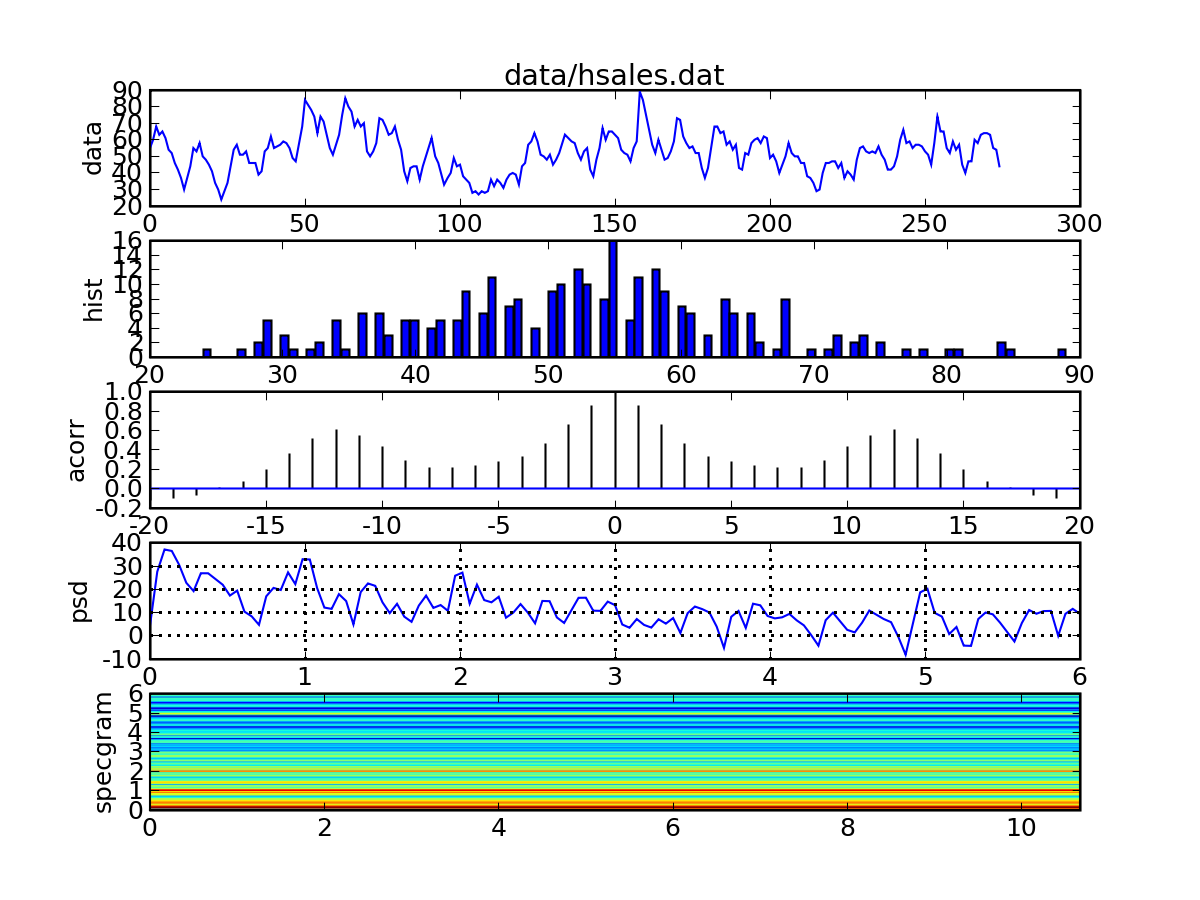
\includegraphics[width=4in]{fig/stats_descriptives}\par\end{centering}

\caption{\label{fig:stats_descriptives}}
\end{figure}
